\chapter{Opis badania}\label{chapter:opis_badania}

\section{Cel i metodologia badań}\label{chapter:cel_i_metodologia_badan}

Przeprowadzenie odpowiednich badań jest kluczowym elementem pracy, który ma na celu znaczące wsparcie odpowiedzi na postawione pytania badawcze.
Po pierwsze, skupiono się na dwóch pierwszych pytaniach badawczych:
\begin{itemize}
    \item PB1: Które metody optymalizacji pozwalają na najlepszą poprawę czasu wykonania funkcji AWS Lambda w ekosystemie Java?
    \item PB2: W jakim stopniu wybrane metody optymalizacji redukują czas zimnego startu funkcji Java w AWS Lambda?
\end{itemize}
Aby udzielić odpowiedzi na powyższe pytania, zdecydowano się na wykonanie testów wydajnościowych funkcji.
Opierały się one na przygotowanych wcześniej funkcjach, które implementowały konkretne metody optymalizacji (opisane w Rozdziale \ref{chapter:wybrane_metody_optimalizacji}).
Specyfikacja poszczególnych funkcji została przedstawiona w kolejnych rozdziałach.
Bazując na wnioskach wyciągniętych w ramach przeglądu literatury (opisanego w Rozdziale \ref{chapter:przeglad_literatury}) zdecydowano się na rozszerzenie badania o wybrane parametry, które mogą wpłynąć na ogólną wydajność usługi.
Były to wielkość pamięci funkcji oraz pomiar zarówno ciepłych, jak i zimnych startów.  

W celu porównania skuteczności wybranych metod opracowano konkretne metryki, które zostały użyte w badaniu:
\begin{enumerate}
    \item Czas działania funkcji podczas ciepłego startu (w milisekundach).
    \item Czas działania funkcji podczas zimnego startu (w milisekundach).
    \item Współczynnik wydajności funkcji.
    \item Koszt działania funkcji (w dolarach amerykańskich).
\end{enumerate}

Pierwsza metryka, czyli czas działania funkcji podczas ciepłego startu jest najprostszym pomiarem.
Określa ona bezpośrednio wydajność funkcji w przypadku większości wywołań.
Dlatego metryka ta pełni kluczową rolę w określeniu efektywności poszczególnych metod.
Aby jednak zawrzeć w badaniu także drugi rodzaj startów (oraz odpowiedzieć na drugie pytanie badawcze), określono kolejną metrykę, czyli czas działania funkcji podczas zimnego startu.
W celu dokonania jego pomiaru, niezbędne jest odpowiednie przygotowanie funkcji, które wymaga większych nakładów pracy w przygotowaniu środowiska badawczego, co zostało opisane w kolejnych rozdziałach.
Pozwala to jednak na rzetelniejsze określenie skuteczności konkretnych metod.
Same zimne starty są uznawane za problematyczne w przypadku użycia Javy w AWS Lambda \cite{9284261}\cite{8605777}.
Dlatego metryka ta jest wymagana, by ująć w badaniu bardziej rzeczywiste przypadki użycia usługi.

Osobna analiza ciepłych i zimnych startów jest jednak niewystarczająca, aby rzetelnie określić efektywność metod w kontekście ich praktycznego użycia.
W momencie działania, funkcje AWS Lambda doświadczają obu typów startów, z dominacją ciepłych startów w przypadku aktywnych funkcji.
Z tego powodu rozszerzono badania o metryki, na które wpływ ma czas działania funkcji podczas obu wariantów uruchomień.
Są to współczynnik wydajności funkcji oraz koszt jej działania.

Na potrzeby pracy został zaproponowany współczynnik wydajności funkcji (WWF). 
Wpływ na niego mają zarówno ciepłe, jak i zimne uruchomienia funkcji.
Aby opracowany współczynnik lepiej odwzorowywał realne użycie usługi AWS Lambda zdecydowano się na wykorzystanie wag, które modyfikują oddziaływanie ciepłych i zimnych startów.
Możliwe jest porównanie skuteczności metod optymalizacji wydajności poprzez porównanie wartości WWF, gdzie im wyższa wartość, tym efektywniejsza jest dana metoda.
Współczynnik wydajności funkcji określony jest wzorem:

\[
\mathrm{WWF} = \frac{1000}{t_c \cdot w_c + t_w \cdot w_w}
\]

gdzie:
\begin{itemize}
  \item \( t_c \) - średni czas zimnego startu funkcji [ms],
  \item \( t_w \) - średni czas ciepłego startu funkcji [ms],
  \item \( w_c \) - waga zimnych startów,
  \item \( w_w \) - waga ciepłych startów.
\end{itemize}

Kolejną metryką łączącą ciepłe i zimne starty jest koszt działania funkcji.
Jest to jeden z głównych elementów wdrożenia technologii bezserwerowych, które rozliczane są w zależności od użycia usług.
W przypadku AWS Lambda jest on określany ze względu na czas działania funkcji, wielkość pamięci oraz liczbę wywołań \cite{awsLambdaPricing}.
Ostatni czynnik nie został zawarty w metryce, gdyż nie jest on zależny od wydajności funkcji.
Dwa pierwsze liczone są jako GB-sekundy, które są iloczynem wielkości pamięci (w GB) i czasu działania funkcji (w sekundach).
Metryka ta jest istotna, gdyż w badaniu zostały zawarte różne wielkości pamięci funkcji.
Z tego względu wartościowy jest także pomiar wpływu poszczególnych metod na wydajność kosztową, na którą składają się zarówno czas działania, jak i wielkość pamięci.
Na potrzeby pracy koszt działania przykładowej funkcji został określony wzorem:

\[
\text{K} = P \cdot M \cdot  r \cdot \left( p_c \cdot d_c + p_w \cdot d_w \right)
\]

gdzie:
\begin{itemize}
  \item \( K \) - całkowity koszt działania funkcji [USD],
  \item \( P \) - cena za jedną GB-sekundę [USD],
  \item \( M \) - pamięć funkcji [GB],
  \item \( r \) - liczba wywołań funkcji na sekundę,
  \item \( p_w \) - udział ciepłych startów (np. 0,95),
  \item \( p_c \) - udział zimnych startów (np. 0,05), gdzie \( p_c = 1 - p_w \),
  \item \( d_c \) - średni rozliczany czas dla zimnych startów (w sekundach),
  \item \( d_w \) - średni rozliczany czas dla ciepłych startów (w sekundach).
\end{itemize}

Kryteria dla PB3:

\begin{enumerate}
    \item Czas budowy artefaktu
    \item Wielkość artefaktu
    \item Dostępność AWS SDK
    \item Wsparcie dla testów
\end{enumerate}
% TODO: opisać badanie w związku z PB3 (czas budowy, dostępność SDK, wielkość artefaktu (?), wsparcie dla testów (?))

\section{Implementacja funkcji}\label{chapter:implementacja_funkcji}

Dla przeprowadzenia badania niezbędne było określenie zadań, które będą realizowane przez funkcję AWS Lambda.
W celu zapewnienia lepszej oceny skuteczności konkretnych metod optymalizacji oraz upodobnienia środowiska badawczego do realnych użyć usługi, przyjęto kilka założeń.
Następnie, stworzono implementację usługi, zgodną z przyjętymi wcześniej zasadami.

Po pierwsze, funkcja powinna wykonywać pewne obliczenia oraz nie być programem zwracającym jedynie tekstową wiadomość (np. ,,Hello World!''). 
Założenie to pozwoli na lepszą weryfikację metod, poprzez realne użycie zaimplementowanego kodu.
Eismann i inni autorzy \cite{eismann2021reviewserverlessusecases} dokonali przeglądu przypadków użycia technologii bezserwerowych.
Wynika z niego, że najczęstsze przypadki użycia to implementacje interfejsu API, procesowanie wydarzeń, zadania wsadowe (ang. batch tasks) oraz wsparcie operacji i monitoring istniejących systemów.
Wszystkie te przypadki wymagają wykonania choćby podstawowych operacji, dlatego stworzenie funkcji wykonującej określone obliczenia pozwoli na analizę metod, w środowisku bardziej zbliżonym do realnych zastosowań.
W przypadku prostych funkcji, które jedynie zwracają pewien tekst niezależny od danych wejściowych, wywołanie skupiłoby się jedynie na procesie inicjalizacji danego narzędzia.

Drugim założeniem jest użycie zewnętrznych zależności, które powinny zostać zawarte w zbudowanym artefakcie.
Wynika ono z dwóch powodów. Po pierwsze, biznesowe użycia AWS Lambda często wymagają zależności zewnętrznych (np. pakietów SDK dla innych usług \cite{eismann2021reviewserverlessusecases}).
Po drugie, wielkość pakietu wdrożeniowego wpływa na wydajność funkcji \cite{8116416}\cite{9095731}.
Zatem aby zwiększyć jego rozmiar i upodobnić ostateczne artefakty do zastosowań praktycznych, zdecydowano się dodać biblioteki zewnętrzne.
Są one jednak zorientowane na konkretnym zadaniu (co zostanie przedstawione w dalszej części rozdziału), a ich liczba nie powinna być zbyt duża.

Po trzecie, funkcja nie powinna używać usług zewnętrznych.
Funkcje bezserwerowe bardzo często integrują się z innymi usługami \cite{eismann2021reviewserverlessusecases}, jednak odrzucono ich użycie w badanych funkcjach.
Wynika to z ryzyka wpływu czynników, które są niezależne od badanych metod, na czas procesowania funkcji.
Mogą to być różnego typu opóźnienia sieciowe (np. w przypadku zapytań do baz danych działających poza infrastrukturą AWS Lambda), które mogą różnić się między wywołaniami.

\begin{figure}[h]
    \centering
    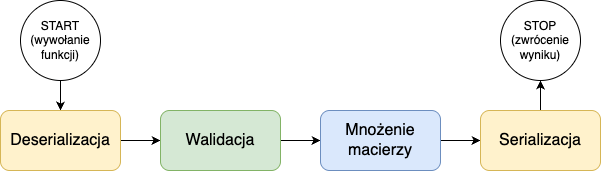
\includegraphics[width=0.95\textwidth]{charts/lambda_workflow.drawio.png}
    \caption{Wizualizacja procesu realizowanego przez badane funkcje AWS Lambda [źródło: opracowanie własne]}
    \label{fig:lambda_workflow}
\end{figure}

Zgodnie z powyższym opracowano zadanie, które będzie realizowane przez funkcje.
Aby utrzymać prostotę implementacji, zdecydowano się na wykonanie przez nią obliczeń, którymi jest mnożenie macierzy.
Są to już jednak wystarczające operacje, które wydłużą czas działania funkcji.
Macierze, które zostaną poddane mnożeniu były przekazywane do funkcji jako dane wejściowe.
Umożliwiło to wykonanie dwóch kolejnych operacji: walidacji oraz deserializacji.
W tym celu użyto zewnętrznych zależności, które pozwoliły na zwiększenie rozmiaru artefaktu.
Biblioteki dla konkretnych języków oraz zastosowań zostały przedstawione w Tabeli \ref{table:lambda_external_dependencies}.
Mimo interoperacyjności Javy i Kotlina, zdecydowano się na użycie bibliotek, które zostały zaimplementowane w konretnym języku używanym w danej funkcji.
Cały proces realizowany przez funkcję AWS Lambda został przedstawiony na Rysunku \ref{fig:lambda_workflow}.
Jego pierwszym elementem była deserializacja danych wejściowych, które zostały przekazane jako napis (typ String) w formacie JSON.
Już odczytane macierze zostały poddane walidacji sprawdzającej ich wielkość, a następnie pomnożone.
Wynik działania został poddany serializacji z powrotem do postaci napisu i zwrócony jako wynik wywołania funkcji.
Cały proces został analogicznie zaimplementowany w każdej z badanych funkcji.

\begin{table}[h!]
    \caption{Zewnętrzne zależności wykorzystane w badanych funkcjach}
    \centering
    \begin{tabularx}{\textwidth}{|X|X|X|} % Wszystkie trzy kolumny o równej szerokości, tabela na całą szerokość tekstu
    \hline
    \textbf{Język programowania} & \textbf{Przeznaczenie}           & \textbf{Nazwa biblioteki} \\ \hline
    \multirow{2}{*}{Java}        & Serializacja i deserializacja    & io.quarkus:quarkus-jackson           \\ \cline{2-3}
                                & Walidacja                        & io.quarkus:quarkus-hibernate-validator \\ \hline
    \multirow{2}{*}{Kotlin}      & Serializacja i deserializacja    & org.jetbrains.kotlinx:kotlinx-serialization-json \\ \cline{2-3}
                                & Walidacja                        & io.konform:konform                    \\ \hline
    \end{tabularx}
    \label{table:lambda_external_dependencies}
\end{table}

W ramach badania przygotowano 7 funkcji, które realizowały wybrane metody optymalizacji wydajności.
Każda funkcja wykorzystywała specyficzne narzędzia, które zostały opisane poniżej, a ich wersje zostały podane w Tabeli \ref{table:lambda_tools_versions}.
Funkcje wykorzystujące język Java używały jej w wersji 21, funkcje oparte o Kotlin używały go w wersji 2.1.0. 
W ramach pracy zrealizowano poniższe warianty:

\begin{itemize}
    \item \textbf{Java JVM} - standardowa implementacja w języku Java, działająca w środowisku JVM, która służy jako baza do analizy skuteczności wybranych metod.
    Została zrealizowana w oparciu framework Quarkus, który wspiera wdrożenia do AWS Lambda \cite{quarkus-docs} i znacząco przyspieszona rozwój oprogramowania.
    Framework został wybrany także z powodu integracji z natywnymi obrazami GraalVM i wsparciem dla usługi SnapStart \cite{quarkus-docs}.
    \item \textbf{Java JVM + SnapStart} - w celu wykorzystania metody SnapStart użyto tej samej implementacji jak w przypadku funkcji Java JVM.
    Funkcja ta działa także z użyciem maszyny wirtualnej Java ale z aktywowaną funkcją SnapStart.
    \item \textbf{Java GraalVM} - implementacja w języku Java, wykorzystująca ten sam kod jak w przypadku dwóch poprzednich funkcji, jednak skompilowany do obrazu natywnego GraalVM.
    W tym celu wykorzystano możliwości frameworka Quarkus oraz niestandardowe środowisko uruchomieniowe (ang. custom runtime) w AWS Lambda.
    \item \textbf{Kotlin JVM} - analogiczna implementacja w języku Kotlin, zrealizowana z użyciem narzędzia http4k zapewniającego integrację z serwisem AWS Lambda \cite{http4kCoreDocs}.
    Narzędzie zostało użyte ze względu na jego oparcie o język Kotlin i natywne wsparcie dla tego języka programowania.
    Następnie funkcja została wdrożona i uruchamiana w środowisku JVM.
    \item \textbf{Kotlin JVM + SnapStart} - funkcja oparta o implementację poprzedniej funkcji, działająca z użyciem maszyny wirtualnej Java i z uruchomioną usługą SnapStart.
    \item \textbf{Kotlin/JS} - implementacja w języku Kotlin, która została następnie transpilowana do języka JavaScript.
    Nie zostały użyte żadne dodatkowe biblioteki (oprócz zależności określonych w Tabeli \ref{table:lambda_external_dependencies}), a komponent oparty jest bezpośrednio o projekt Kotlin Multiplatform.
    We wdrożeniu funkcji użyto środowiska Node.js, oferowanego przez AWS Lambda \cite{awsLambdaDocs}.
    \item \textbf{Kotlin/Native} - implementacja w języku Kotlin, która została następnie skompilowana do binarnego pliku natywnego i wdrożona z użyciem niestandardowego środowiska uruchomieniowego (ang. custom runtime).
    Funkcja wykorzystuje bibliotekę kotlin-native-aws-lambda-runtime \cite{kotlinNativeLambdaRuntime}, która zapewnia możliwość budowy artefaktów natywnych i wsparcie obsługi żądań.
    Biblioteka oparta jest w całości o język Kotlin, framework Ktor oraz możliwości Kotlin Multiplatform. 
\end{itemize}

\begin{table}[h!]
    \caption{Biblioteki oraz frameworki użyte podczas implementacji badanych funkcji}
    \centering
    \begin{tabular}{|l|l|l|}
    \hline
    \textbf{Rodzaj funkcji}           & \textbf{Użyta biblioteka/framework}                               & \textbf{Wersja} \\ \hline
    Java JVM                          & \multirow{3}{*}{io.quarkus:quarkus-amazon-lambda} & \multirow{3}{*}{3.17.5}   \\ \cline{1-1}
    Java JVM + SnapStart              &                                                  &                           \\ \cline{1-1}
    Java GraalVM                      &                                                  &                           \\ \hline
    Kotlin JVM                        & \multirow{2}{*}{http4k-serverless-lambda}         & \multirow{2}{*}{6.9.0.0}  \\ \cline{1-1}
    Kotlin JVM + SnapStart            &                                                  &                           \\ \hline
    Kotlin/JS                         & Brak                                             & Brak                      \\ \hline
    Kotlin/Native                     & io.github.trueangle:lambda-runtime               & 0.0.2                     \\ \hline
    \end{tabular}
    \label{table:lambda_tools_versions}
\end{table}

Wartym zaznaczenia w kontekście implementacji funkcji są zdolności Kotlin Multiplatform (opisane w Rozdziale \ref{chapter:kotlin_multiplatform}), które zostały użyte podczas tworzenia funkcji.
Główna część funkcji, tj. serializacja, walidacja, mnożenie oraz deserializacja, zostały umieszczone w module commonMain oraz współdzielone między wszystkie docelowe platformy.
Następnie w modułach dla danych platform (jvmMain, jsMain oraz nativeMain) została zaimplementowane obsługa zapytania oraz wywołania funkcji z części commonMain.
Pozwoliło to na badanie oparte o dokładnie ten sam kod, który został użyty w każdej z badanych funkcji.
Możliwości współdzielenia kodu miały także wpływ na wybór bibliotek do walidacji oraz serializacji, które musiały wspierać kompilację dla każdej z badanych platform.

\section{Wdrożenie funkcji}\label{chapter:wdrożenie_funkcji}

Kolejnym elementem niezbędnym do przeprowadzenia badania było wdrożenie testowanych funkcji już na platformę chmurową.
Etap ten wymagał utworzenia także niezbędnej infrastruktury ciągłej integracji oraz procesu wdrażania, co umożliwiło automatyzację procesu budowy i aktualizacji funkcji AWS Lambda. 
Proces ten został zrealizowany z wykorzystaniem narzędzi infrakstruktury jako kod (ang. Infrastructure as a Code), co zapewniło powtarzalność i spójność środowiska testowego.
Przygotowanie potoku ciągłego integracji jest także niezbędne w przypadku używania środowisk deweloperskich z procesorami o architekturze ARM64.
Funkcje zostały wdrożone w architekturze x86-64, zatem do budowy artefaktów potrzebne było użycie maszyn operujących także w tym typie procesora.

Cały proces budowy artefaktów oraz ich wdrażania został zautomatyzowany z użyciem GitHub Actions.
Do wytworzenia artefaktu użyto narzędzia Gradle, który pozwał na uruchomienie odpowiedniego zadania dla każdej z zaimplementowanych funkcji.
Odpowiadało ono za kompilację kodu źródłowego, czego wynikiem były pliki gotowe do uruchomienia programu.
Dla każdej z przygotowanych funkcji utworzono odpowiedni krok w procesie GitHub Actions, który uruchamiał proces budowy dla danej platformy i docelowej architektury x86-64 (np. Java JVM czy Kotlin/JS).
Stworzone w ten sposób pliki były następnie przekazywane do drugiego kroku, który odpowiadał za wgranie ich do usługi S3 (ang. Simple Storage Service).
Przechowywane tak pakiety były już gotowe do użycia w wdrażanych funkcjach AWS Lambda.
Dodatkowo, opisany proces ciągłej integracji pozwolił na pomiar czasu budowy funkcji, co jest istotne w odpowiedzi na postawione pytania badawcze i zostało zawarte w wynikach badania.
Wielkość artefaktów została zmierzona jako wielkośc plików przechowywanych w usłudze S3.

Kolejnym etapem było wdrożenie przechowywanych w serwisie S3 artefaktów jako funkcje AWS Lambda.
W tym celu użyto narzędzia Terraform, które pozwala na wdrożenie infrastruktury chmurowej w oparciu o kod.
W ramach konfiguracji Terraform dla każdej instancji AWS Lambda określono nazwę funkcji, lokalizację artefaktu w usłudze S3, sygnaturę wywoływanej metody (tj. pełną ścieżkę do metody, która będzie wywoływana po otrzymaniu zdarzenia), środowisko wykonawcze oraz czy funkcja aktywuje usługę SnapStart.
Środowiska wykonawcze, w których uruchomiano poszczególne funkcje, zostały przedstawione w Tabeli \ref{table:lambda_runtimes}.
Każda funkcja została wdrożona dla następujących wielkości pamięci: 128 MB, 256 MB, 512 MB, 1024 MB oraz 2048 MB.

Istotnym faktem dla wdrożenia funkcji z użyciem Kotlin/Native jest potrzeba utworzenia dodatkowej warstwy AWS Lambda (ang. lambda layer).
Warstwy te stanowią archiwum w formacie .zip, zawierające dodatkowy kod lub dane, takie jak zależności biblioteczne, niestandardowe środowiska wykonawcze czy pliki konfiguracyjne.
Dla funkcji Kotlin/Native zbudowano warstwę, która zawierała zależność libcrypt.
Biblioteka ta nie jest domyślnie dostępna w dystrybucji Amazon Linux 2023, jednak jest wymagana do działania przez technologię użytą w implementacji Kotlin/Native \cite{kotlinNativeLambdaRuntime}.
Potrzeba ta wynikała z użycia niestandardowego środowiska uruchomieniowego, co może wpłynąć na jakość procesu rozwoju oprogramowania i powinny być wzięte pod uwagę podczas użycia takich środowisk.

\begin{table}[h!]
    \caption{Środowiska wykonawcze użyte w badanych funkcjach AWS Lambda}
    \centering
    \begin{tabular}{|l|l|}
    \hline
    \textbf{Rodzaj funkcji}           & \textbf{Identyfikator środowiska wykonawczego}                               \\ \hline
    Java JVM                          & java21                                                      \\ \hline
    Java JVM + SnapStart              & java21                                                      \\ \hline
    Java GraalVM                      & provided.al2023                                              \\ \hline
    Kotlin JVM                        & java21                                                      \\ \hline
    Kotlin JVM + SnapStart            & java21                                                      \\ \hline
    Kotlin/JS                         & nodejs22.x                                                   \\ \hline
    Kotlin/Native                     & provided.al2023                                              \\ \hline
    \end{tabular}
    \label{table:lambda_runtimes}
\end{table}

\section{Środowisko badawcze}\label{chapter:srodowisko_badawcze}

W celu pomiaru wartości metryk (określonych w Rozdziale \ref{chapter:cel_i_metodologia_badan}) przygotowano odpowiednią infrastrukturę chmurową wdrożoną w środowisku AWS.
Jej zadaniem było odpowiednie przygotowanie badanych funkcji, ich uruchomienie oraz zebranie wyników pomiarowych.
Architektura środowiska badawczego została przedstawiona na Rysunku \ref{fig:experiment_architecture} oraz dokładnie opisana w poniższym rozdziale.
Przygotowanie takiego środowiska pozwoliło na automatyczne przeprowadzenie eksperymentu oraz ułatwia jego ewentualne powtórzenie.
Do wdrożenia środowiska wykorzystano bezserwerowe usługi oferowane przez AWS (m.in. AWS Lambda oraz serwisy integrujące się z nią).

Głównym zadaniem przygotowanego środowiska badawczego jest wywołanie przygotowanych wcześniej funkcji, aby przeprowadzić serię pomiarów ich wydajności.
W tym celu środowisko zostało zaprojektowane tak, aby umożliwić kontrolowane wykonanie funkcji po określonej liczbie tzw. zimnych startów (ang. cold starts) oraz ciepłych startów (ang. warm starts). 
Po każdym wywołaniu, środowisko odpowiada za zebranie kluczowych metryk wydajnościowych. 
Zebrane wyniki są następnie przetwarzane i agregowane, co pozwala na generowanie finalnego pliku w formacie JSON, który stanowi podstawę do dalszej analizy badanych metod.

Kluczowym aspektem badania jest rozróżnienie między zimnym a ciepłym startem funkcji.
Dlatego niezbędne było odpowiednie przygotowanie badanej funkcji przed jej wywołaniem, co pozwoliło osiągnąć oczekiwany rodzaj startu.
Inicjalizacja ta różniła się od rodzaju startu oraz od faktu, czy aktywowana jest usługa SnapStart.
W tym celu przygotowano specjalną funkcję AWS Lambda (,,funkcję wywołującą'' oznaczoną numerem 3 na Rysunku \ref{fig:experiment_architecture}) otrzymującą jako dane wejściowe kod ARN (ang. Amazon Resource Name) badanej funkcji AWS Lambda, która ma zostać przygotowana i wywołana.

\begin{figure}[h]
    \centering
    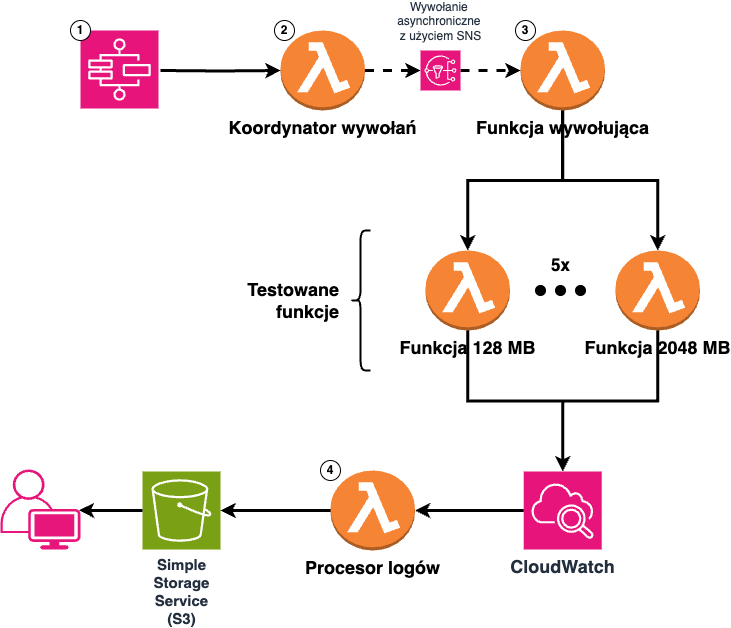
\includegraphics[width=1\textwidth]{charts/experiment-architecture.drawio.png}
    \caption{Architektura środowiska badawczego [źródło:~opracowanie~własne]}
    \label{fig:experiment_architecture}
\end{figure}

W celu wiarygodnego pomiaru czasu zimnego startu standardowej funkcji Lambda (bez aktywowanej funkcji SnapStart), funkcja wywołująca przed każdym pomiarem celowo modyfikuje konfigurację badanej funkcji poprzez zmianę wartości jej zmiennej środowiskowej. 
Ta operacja wymusza na platformie AWS Lambda odrzucenie ewentualnie istniejącego, gotowego do użycia środowiska wykonawczego i utworzenie nowego, co dokładnie symuluje warunki zimnego startu \cite{awsLambdaDocs}.
Ciepłe starty dla funkcji standardowych mierzone są poprzez kolejne, następujące po sobie wywołania tej samej, już ,,rozgrzanej'' instancji funkcji, bez wprowadzania zmian w jej konfiguracji.

Inaczej realizowane jest przygotowanie do testów dla funkcji z aktywowaną opcją SnapStart.
Wynika to z przygotowywania migawek stanu przez AWS Lambda dla każdej z utworzonych wersji funkcji.
Aby zatem precyzyjnie zmierzyć czas zimnego startu funkcji wykorzystującej SnapStart, zastosowano metodę polegającą na opublikowaniu kolejnych wersji badanej funkcji. 
Każda z tak przygotowanych wersji jest następnie poddawana jednokrotnemu wywołaniu. 
Takie podejście gwarantuje, że każde zarejestrowane uruchomienie stanowi pomiar czasu potrzebnego na odtworzenie funkcji ze stanu zapisanego w migawce, rzetelnie testując mechanizm SnapStart. 
Po zakończeniu dedykowanej serii pomiarów, wszystkie wersje funkcji, które zostały utworzone wyłącznie na potrzeby tego etapu badania są usuwane. 
Metody te pozwalają na dokładne wywołania funkcji, które uruchamiane są zgodnie z planem badań.

Kolejnym elementem badania jest odpowiednie uruchomienie funkcji wywołującej.
Proces ten został zaprojektowany w taki sposób, aby uniknąć przekraczania limitów API AWS Lambda, co było problemem podczas tworzenia pierwszych iteracji środowiska badawczego.
Procedura opierała się m.in. na oczekiwaniu pomiędzy kolejnymi operacjami.
Po pierwsze, w funkcji wywołującej pomiędzy kolejnymi aktualizacjami oraz wywołaniami funkcji, program jest zatrzymywany.
Sama funkcja wywołująca nie była uruchamiała pomiaru wszystkich funkcji jednocześnie.
Do zarządzania pomiarami stworzono funkcję koordynatora wywołań (oznaczoną numerem 2 na Rysunku \ref{fig:experiment_architecture}), której rolą jest wybór funkcji przeznaczonych do analizy na podstawie określonych kryteriów, takich jak użycie mechanizmu SnapStart czy język implementacji.
Pozwala to na zmniejszenie badanych jednocześnie funkcji, a co za tym idzie zapytań do API.

Dla każdej z wybranych funkcji, koordynator przygotowuje i wysyła wiadomość do tematu w usłudze Amazon Simple Notification Service (SNS).
Wiadomość ta zawiera identyfikator ARN badanej funkcji oraz pożądany typ startu (zimny lub ciepły), inicjując w ten sposób funkcję wywołującą.
Istotnym elementem działania koordynatora jest również wprowadzenie kontrolowanego opóźnienia pomiędzy publikacją kolejnych wiadomości, co ma na celu rozłożenie obciążenia w czasie i zapobieganie wspomnianym problemom z limitami usług AWS.

Pomiędzy kolejnymi wywołaniami funkcji koorydnatora także zastosowano określone przerwy.
W tym celu użyto usługi AWS Step Functions (oznaczonej numerem 1 na Rysunku \ref{fig:experiment_architecture}), która pozwala na tworzenie i wizualizację procesów wchodzących w interakcję z różnymi serwisami AWS.
Jej zadaniem było iteracyjne uruchamianie koordynatora dla kolejnych kombinacji parametrów (języka implementacji, aktywacji SnapStart oraz typu startów).
Po każdym uruchomieniu następuje 30 minutowa przerwa, podczas której usługa czeka aby najnowsze wywołanie koordynatora zostało zakończone.
Wydłuża to znacząco czas potrzebny na wykonanie badanie, jednak pozwala na uniknięcie zbytniego obciążenia API, a co za tym idzie blokady kolejnych wywołań.

Ostatnim elementem badania była agregacja wyników pomiarów.
W tym celu użyto usługi AWS CloudWatch, który pozwala na przesyłanie wszystkich logów wywoływanych funkcji.
Po każdym wywołaniu, funkcja AWS Lambda automatycznie tworzy raport, który zawiera:
\begin{itemize}
    \item czas wykonania,
    \item opłacony czas wykonania,
    \item czas inicjalizacji,
    \item czas odtworzenia stanu z migawki (w przypadku aktywnego SnapStart)
    \item opłacony czas odtworzenia stanu z migawki (w przypadku aktywnego SnapStart)
\end{itemize}
Wszystkie te dane są następnie przesyłane do usługi CloudWatch. 
Aby móc dokonać analizy wyników niezbędne było ich zagregowanie i zapisanie (np. w pliku JSON).
Wykorzystano do tego przygotowaną funkcję procesora logów (oznaczoną numerem 4 na Rysunku \ref{fig:experiment_architecture}), która pobierała logi z raportami z usługi CloudWatch, transformowała oraz zapisywała w pliku JSON.
Następnie plik był wgrywany do usługi S3, co pozwalało na pobranie przez użytkownika.
Tak przygotowana agregacja logów umożliwiła następnie niezbędną analizę wyników badania.
